\paragraph{}{
	Le sélecteur de registres permet de déterminer le registre
	dans lequel on va lire ou écrire un octet. Son circuit électronique
	est présenté à la figure \ref{selec_reg_circ}.
	Sont fonctionnement est relativement simple, on ne s’attardera donc
	pas dessus.
}

\begin{figure}[!h]
	\centering
	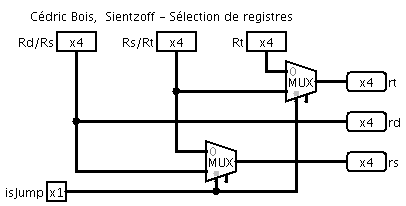
\includegraphics[scale=0.8,origin=c]{circuits/selec_reg.png}
	\caption{
		\label{selec_reg_circ}
		Sch\'{e}ma \'{e}lectronique pour la s\'{e}lection de registres
	}
\end{figure}

\paragraph{}{
	Maintenant que nous sommes en capacité de choisir un registre
	et l'opération qu'on souhaite y faire, réalisons le banc de
	registres.
}